\StartOf{Lecture 15}

\Today{(1) $M>2$ FSK Prob.\ Error, (2) Modulation Comparison}

\announcements{
}

\section{$M$-ary FSK Probability of Error}

\subsection{$M$-ary Non-Coherent FSK}

For $M$-ary non-coherent FSK, the derivation in the Proakis \& Salehi book, section 7.6.9, provides an exact expression for the probability of error in $M$-ary FSK.  The result is that
\[
\PR{\mbox{symbol error}} = \sum_{n=1}^{M-1} (-1)^{n+1} {M-1 \choose
n} \frac{1}{n+1} e^{-\log_2 M \frac{n}{n+1}\Ebno},
\]
and
\[
  \PR{\mbox{error}}_{M-nc-FSK} = \frac{M/2}{M-1}\PR{\mbox{symbol error}}.
\]
See Figure \ref{F:BER_NCFSK_Mary}.

\textit{Proof Summary}:  Our non-coherent receiver finds the energy in each frequency.  These energy values no longer have a Gaussian distribution (due to the squaring of the amplitudes in the energy calculation).  They instead are either Rician (for the transmitted frequency) or Rayleigh distributed (for the ``other'' $M-1$ frequencies).  The probability that the correct frequency is selected is the probability that the Rician random variable is larger than all of the other random variables measured at the other frequencies.

\begin{figure}[htbp]
  \centerline{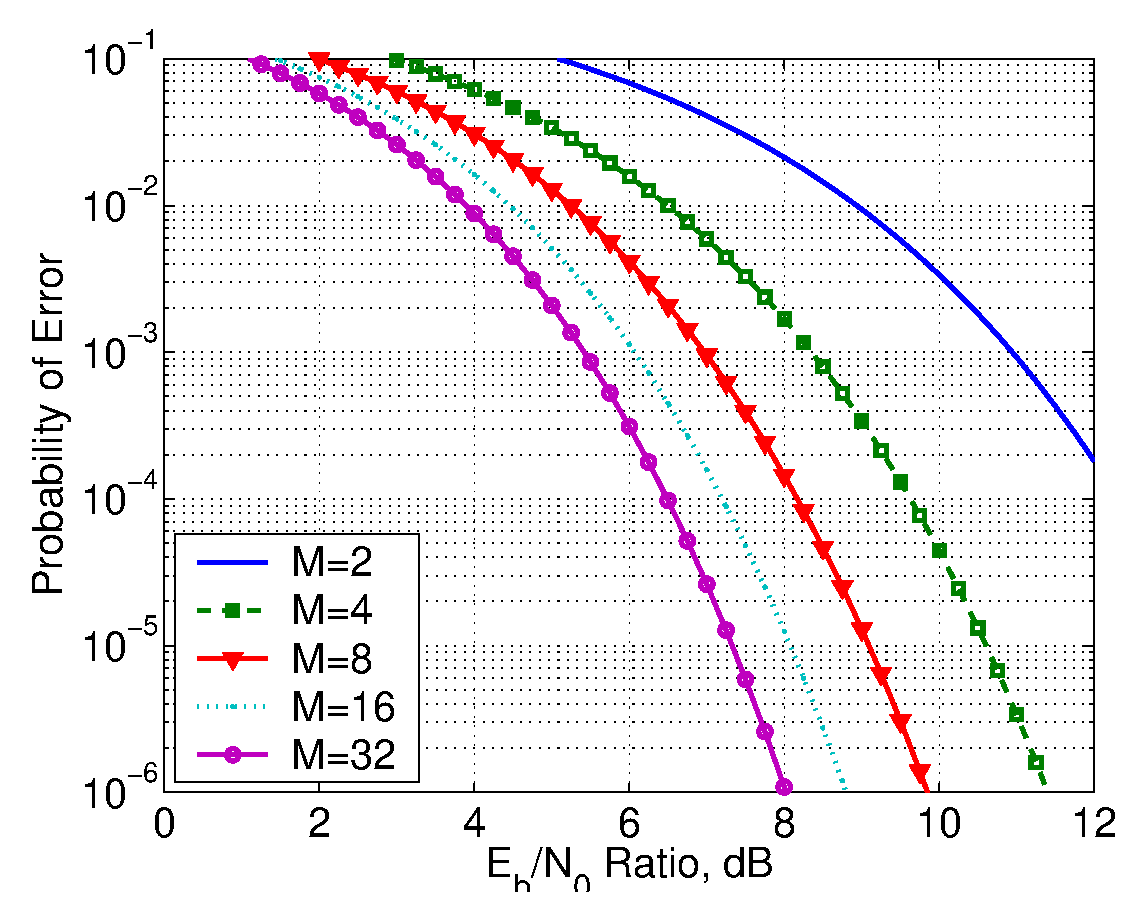
\includegraphics[width=3in]{../images/plotBER_NCFSK_Mary.eps} }
  \caption{Probability of bit error for non-coherent reception of M-ary FSK.}
  \label{F:BER_NCFSK_Mary}
\end{figure}

\Example{Probability of Error for Non-coherent $M=2$ case}  Use the
above expressions to find the $\PR{\mbox{symbol error}}$ and
$\PR{\mbox{error}}$ for binary non-coherent FSK.

\Solution{
\[
\PR{\mbox{symbol error}} =  \PR{\mbox{bit error}} =
\frac{1}{2}e^{-\frac{1}{2}\Ebno}
\]
}

\subsection{$M$-ary FSK Coherent Receiver}

\begin{figure}
    \centering
    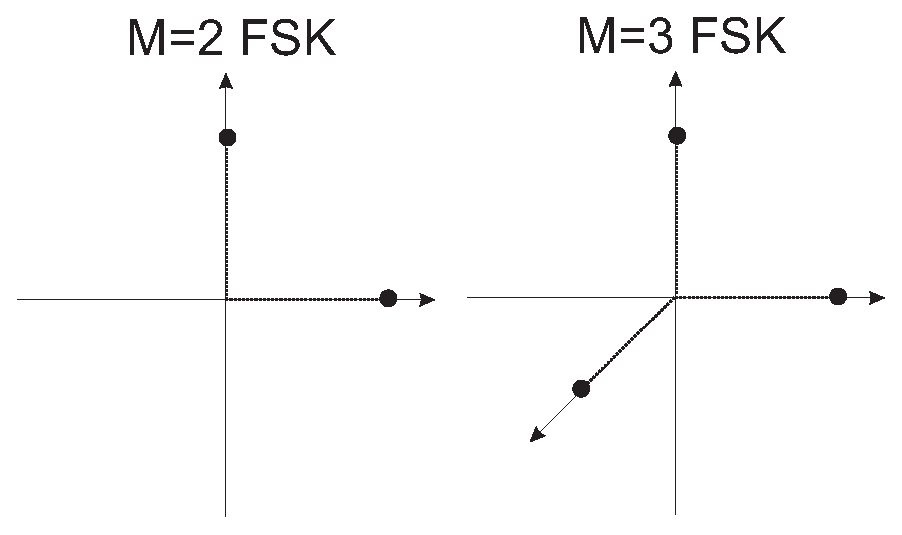
\includegraphics[width=0.5\textwidth]{../images/FSK-signalSpaceDiagram.eps}
    \caption{Constellation for $M=2$, $M=3$ FSK.}
    \label{F:FSK_constellation}
\end{figure}

For $M$-ary FSK with $M>2$, we don't have an exact expression for the probability of symbol error.  Instead, we use the union bound.  How many neighbors does each symbol have?  You can the constellation visually when $M=2$ or $M=3$ (in Figure \ref{F:FSK_constellation}).  For $M>3$, consider plotting any three dimensions of the constellation, and one of the three axes is symbol 0. You can see that both other symbols contribute a plane that contributes to the decision region of the symbol 0.  This is true regardless of which other symbols were chosen.  Thus each symbol has $M-1$ neighbors! 

The distance between neighbors is always $d=\sqrt{2}A$, and the average energy per symbol is $\En_s = A^2$, which means that $\En_b = A^2 / \log_2 M$.  Thus:
\begin{equation}
    \PR{\mbox{symbol error}} \le 
      (M-1) \Q{ \sqrt{\log_2 M \frac{\En_b }{N_0}}}
\end{equation}

Note however that one cannot do Gray encoding on the bits assigned to the $M$ symbols.  For symbol $i$, all $M-1$ other symbols are neighbors to it, and they are all equally distant from $i$.  Thus when a symbol error is made, it is equally likely to be to symbol $j\neq i$.  What is the average number of bit errors made when a symbol error is made?  

The Proakis \& Salehi book provides a derivation for the result, which is:
\begin{equation}
    \PR{\mbox{bit error}} = 
      \frac{M/2}{M-1} \PR{\mbox{symbol error}} 
    \le 
      \frac{M}{2} \Q{ \sqrt{(\log_2 M) \frac{\En_b }{N_0}}}.
\end{equation}

Here is a short argument about why we get the result we see in the Proakis \& Salehi handout: If I randomly pick any symbol, it will have $(\log_2 M)/2$ bit errors per symbol.  However, this includes the correct symbol.  Since we need to exclude the correct symbol, we need to multiply by a factor of $M/(M-1)$, that is $\frac{M\log_2 M}{(M-1) 2}$ bit errors per symbol.  Next, because this is the number of bit errors per symbol, we divide by $\log_2 M$ to get the number of bit errors per bit.  That is, $\frac{M/2}{M-1}$.


\section{Fidelity Comparison: $\PR{\mbox{error}}$ vs.~$\Ebno$}


Main modulations which we have evaluated probability of error vs.
$\Ebno$:
\begin{enumerate}
  \item M-ary PAM, including Binary PAM or BPSK, OOK, DPSK.
  \item M-ary PSK, including QPSK.
  \item Square QAM
  \item Non-square QAM constellations
  \item FSK, M-ary FSK
\end{enumerate}

In this part of the lecture we will break up into groups and
derive: (1) the probability of error and (2) probability of symbol
error formulas for these types of modulations.

\begin{table}
\begin{tabular}{|l|cc|}
\hline
 \bf Name & \bf $\PR{\mbox{symbol error}}$ & \bf $\PR{\mbox{bit error}}$ \\
\hline
 BPSK & $=\Q{ \sqrt{\frac{2\En_b }{N_0}}}$ & same \\
 OOK  & $=\Q{ \sqrt{\frac{\En_b }{N_0}}}$ & same \\
 DPSK & $=\frac{1}{2} \exp\left( -\Ebno \right)$ & same \\
 M-PAM & $= \frac{2(M-1)}{M} \Q{\sqrt{\frac{6 \log_2 M}{M^2-1} \frac{\En_b}{N_0}}}$ & 
         $\approx \frac{1}{\log_2 M} \PR{\mbox{symbol error}}$\\
 QPSK &  & $=\Q{ \sqrt{\frac{2\En_b }{N_0}}}$ \\
 M-PSK &  $\le 2 \Q{\sqrt{2 (\log_2 M)\sin^2(\pi/M) \frac{\En_b }{N_0}}}$  & $\approx \frac{1}{\log_2 M} \PR{\mbox{symbol error}}$ \\
% 4-PSK &  $\le 2 \Q{\sqrt{2  \frac{\En_b }{N_0}}}$  & $\approx \frac{1}{\log_2 M} \PR{\mbox{symbol error}}$ \\
 Square M-QAM &  & 
         $\approx \frac{4}{\log_2 M} \frac{(\sqrt{M}-1)}{\sqrt{M}} \Q{\sqrt{\frac{3 \log_2 M}{M-1} \frac{\En_b}{N_0}}}$ \\
 2-non-co-FSK & $=\frac{1}{2} \exp \left[- \frac{\En_b}{2N_0} \right]$ & same \\
 M-non-co-FSK & $=\sum_{n=1}^{M-1}  ({M-1 \atop n})  \frac{(-1)^{n+1}}{n+1} \exp \left[ -\frac{n \log_2 M}{n+1} \Ebno\right]$ 
              & $= \frac{M/2}{M-1} \PR{\mbox{symbol error}}$ \\  % \left( \begin{array}{c} M-1 \\  n \end{array} \right)
 2-co-FSK & $=\Q{\sqrt{\frac{\En_b}{N_0}}}$ & same \\
 M-co-FSK & $\le (M-1) \Q{ \sqrt{\log_2 M \frac{\En_b }{N_0}}}$ 
              & $= \frac{M/2}{M-1} \PR{\mbox{symbol error}}$ \\
\hline
\end{tabular}
\caption{Summary of probability of bit and symbol error formulas for several modulations.}
\end{table}  


See also Rice Section 6.3



\subsection{Bandwidth Efficiency Comparison}

We've talked about measuring data rate in bits per second. We've
also talked about Hertz, \ie, the quantity of spectrum our signal
will use.  Typically, we can scale a system, to increase the bit
rate by decreasing the symbol period, and correspondingly increase
the bandwidth.  These two have a linear proportional relationship.

\Definition{Bandwidth efficiency}{ The bandwidth efficiency, typically denoted $\eta$, is the ratio of bits per second to bandwidth:
\[
  \eta = R_b/B_T
\]
}
Bandwidth efficiency depends on the definition of ``bandwidth''.  Since it is usually used for comparative purposes, we just make sure we use the same definition of bandwidth throughout a comparison.

The key figure of merit:  bits per second / Hertz, \ie, bps/Hz.

\subsubsection{PSK, PAM and QAM}

In these three modulation methods, the bandwidth is largely
determined by the pulse shape.  For root raised cosine filtering,
the null-null bandwidth is $1+\alpha$ times the bandwidth of the
case when we use pure sinc pulses.  The transmission bandwidth (for
a bandpass signal) is
\[
  B_T = \frac{1+\alpha}{T_{s}}
\]
Since $T_{s}$ is seconds per symbol, we divide by $\log_2 M$ bits
per symbol to get $T_b = T_{s} / \log_2 M$ seconds per bit, or
\[
  B_T = \frac{(1+\alpha)R_b}{\log_2 M}
\]
where $R_b = 1/ T_b$ is the bit rate.

Bandwidth efficiency is then
\[
  \eta = R_b/B_T = \frac{\log_2 M}{1+\alpha}
\]
See Table \ref{T:BW_Efficiency} for some numerical examples.

\begin{table}
  \centering
\begin{tabular}{|l|ccc|}
  \hline
  $\eta$ & $\alpha=0$ & $\alpha=0.5$ & $\alpha=1$ \\
  \hline
  BPSK   & 1.0        & 0.67         & 0.5 \\
  QPSK   & 2.0        & 1.33         & 1.5 \\
  16-QAM & 4.0        & 2.67         & 2.0 \\
  64-QAM & 6.0        & 4.0          & 3.0 \\
  \hline
\end{tabular}
  \caption{Bandwidth efficiency of PSK and QAM modulation methods
  using raised cosine filtering as a function of $\alpha$.}\label{T:BW_Efficiency}
\end{table}


\subsubsection{FSK}

We've said that the bandwidth of FSK is,
\[
B_T = (M-1) \Delta f + 2B
\]
where $B$ is the one-sided bandwidth of the digital baseband signal.
For the null-to-null bandwidth of  raised-cosine pulse shaping,
$2B=(1+\alpha)/T_{s}$. So,
\[
B_T = (M-1) \Delta f + (1+\alpha)/T_{s} = \frac{R_b}{\log_2 M}
\left\{(M-1)\Delta f T_{s} + (1+\alpha) \right\}
\]
since $R_b = 1/T_{s}$ for
\[
  \eta = R_b/B_T = \frac{\log_2 M}{(M-1)\Delta f T_{s} + (1+\alpha)}
\]
If $\Delta f = 1/T_s$ (required for non-coherent reception),
\[
  \eta = \frac{\log_2 M}{M+\alpha}
\]


\subsection{Bandwidth Efficiency vs.~$\Ebno$}

For each modulation format, we have quantities of interest:
\begin{itemize}
  \item Bandwidth efficiency, and
  \item Energy per bit ($\Ebno$) requirements to achieve a given
  probability of error.
\end{itemize}

\Example{Bandwidth efficiency vs.~$\Ebno$ for $M=8$ PSK} What is the
required $\Ebno$ for 8-PSK to achieve a probability of bit error of
$10^{-6}$?  What is the bandwidth efficiency of 8-PSK when using
50\% excess bandwidth?

\Solution{Given in Rice Figure 6.3.5 (Figure 6.13?) to be about 14 dB, and 2.}

We can plot these (required $\Ebno$, bandwidth efficiency) pairs.
 See Rice Figure 6.3.6.